\documentclass{article}
\usepackage{geometry}
\geometry{margin=1in}
\usepackage{tabularx}
\usepackage{booktabs}
\usepackage{lmodern}
\usepackage[spanish]{babel}
\decimalpoint
\usepackage{amsmath}
\usepackage{amsfonts}
\usepackage{amssymb}
\usepackage{graphicx}
\usepackage{float}  % Paquete para controlar la posición de las imágenes, se usa [H] en las imágenes
\renewcommand{\figurename}{Imagen}  % Cambia "Figura" por "Imagen"

\usepackage{caption}
\usepackage{placeins}
\usepackage{ragged2e} % para justificar textos
\usepackage{array} % Permite definir alineaciones personalizadas en tablas
\usepackage{booktabs} % Para mejorar la estética de la tabla 
\usepackage{bm} % se usa para poner negritas en expresiones matemáticas
\usepackage{xcolor}  % paquete xcolor para poner color

\usepackage{hyperref} % para navegar sobre el contenido
% Cambia el nombre del índice a "Contenido"
\addto\captionsspanish{\renewcommand{\contentsname}{Contenido}}

\usepackage{listings}
\usepackage{xcolor}

\lstdefinelanguage{R}{
	morekeywords={if, else, repeat, while, function, for, in, next, break},
	otherkeywords={<-, <<-},
	sensitive=true,
	morecomment=[l]{\#}, % ← Aquí se define que # es comentario en R
	morestring=[b]",
	morestring=[b]'
}

\lstset{
	language=R,
	basicstyle=\ttfamily\footnotesize,
	keywordstyle=\color{blue},
	commentstyle=\color{gray},
	stringstyle=\color{red},
	backgroundcolor=\color{white},
	frame=single,
	breaklines=true,
	showstringspaces=false,
	escapeinside={(*@}{@*)} % opcional para insertar LaTeX dentro del código
}


%\title{Tipos de datos espacio temporales: \\
	
%\author{}
%\date{}

\begin{document}
	
	% Desactiva la numeración en la portada
	\pagenumbering{gobble}
	
	\begin{titlepage}
		
		\begin{figure}[H]
			\centering
			
\includegraphics[width=0.8\textwidth]{uami1.png}  
		\end{figure}
		
		\begin{center}
			\LARGE \textbf{Universidad Autónoma Metropolitana} \\[0pt]
			\LARGE \textbf{Unidad Iztapalapa} \\[24pt]
			
			\Large Maestría en Matemáticas Aplicadas e Industriales (MCMAI) \\[24pt]
			
			\Large \textbf{Proyecto final - Taller de modelado II Parte 1} \\[12pt]
			

			Profesor: Dr. Alejandro Román Vásquez \\[8pt]
			Alumnos:\\[12pt]
			\qquad Brandon Eduardo Antonio Gómez \\[6pt]
			\qquad Alan Badillo Salas \\[64pt]
			\large 01 de Julio de 2025 \\[24pt]
			
		\end{center}
	\end{titlepage}
	
	% Desactivar numeración en la tabla de contenido
	\pagenumbering{gobble}
	
	\newpage
	\tableofcontents  
	\newpage
	
	% Iniciar numeración en la Sección 1
	\pagenumbering{arabic}
	
	
	%\maketitle
	
	\section{Fase 1 - Adquisición de los datos}
	\subsection{Objetivo}
	
	El objetivo del proyecto final consiste en aplicar la metodología sobre modelos de aprendizaje estadístico para construir un modelo de clasificación empleando el conjunto de datos \textbf{Adult}, en donde la predicción consiste en determinar si los ingresos de una persona superan los 50000 dólares al año.
	
	\subsection{Introducción}
	
	Al empezar con el pre-procesamiento de los datos nos percatamos de que falta el encabezado en la columnas, por lo que se agregamos los nombres de las columnas al dataframe. \\
	
	
	El conjunto de datos contiene 32561 registros y 15 columnas (variables), las cuales son:
	
	\begin{enumerate}
		\item age: edad (numérico).
		\item Worlclass, clase de trabajo: Privado,(categórico) Autónomo-no-inc, Autónomo-inc, Federal-gov, Local-gov, Estatal-without-pay, gov, (Sin sueldo, Nunca-trabajó.) (categórico)
		\item fnlwgt: Final Weight. Es un peso de muestra (sampling weight) asignado por la Oficina del Censo de EE.UU. Se usa para extrapolar los datos de la muestra a toda la población estadounidense (numérico)
		\item education: Bachelors, Some-college, 11th, HS-grad, Prof-school, Assoc-acdm, Assoc-voc, 9th, 7th-8th, 12th, Masters, 1st-4th, 10th, Doctorate, 5th-6th, Preschool. (categórico)
		\item education-num: (numérico).
		\item marital-status: Married-civ-spouse, Divorced, Never-married, Separated, Widowed, Married-spouse-absent, Married-AF-spouse.(categórico)
		\item occupation: Apoyo técnico, Reparación artesanal, Otros servicios, Ventas, Directivo, Profesional especializado, Manipulador-limpiador, Operador de maquinaria, Administrativo, Agricultor-pescador, Transporte, Servicio doméstico privado, Servicio de protección, Fuerzas armadas.(categórico)
		\item relationship (relación): Esposa, Hijo propio, Esposo, No familiar, Otro pariente, Soltero.(categórico)
		\item race: Blanco, Asiático-Pacífico-Islandés, Amerindio-Esquimal, Otro, Negro.(categórico)
		\item sex: Mujer, Hombre.(categórico)
		\item capital-gain (plusvalía): (numérico)
		\item capital-loss (minusvalía): (numérico)
		\item Hours-per-week (horas-semana): (numérico).
		\item native-country (país-nativo): Estados Unidos, Camboya, Inglaterra, Puerto Rico, Canadá, Alemania, EE.UU. periférico (Guam-USVI-etc.), India, Japón, Grecia, Sur, China, Cuba, Irán, Honduras, Filipinas, Italia, Polonia, Jamaica, Vietnam, México, Portugal, Irlanda, Francia, República Dominicana, Laos, Ecuador, Taiwán, Haití, Colombia, Hungría, Guatemala, Nicaragua, Escocia, Tailandia, Yugoslavia, El Salvador, Trinad \& Tobago, Perú, Hong, Holanda. (categórico)
		\item Income : ingreso (será la variable respuesta $Y$) (categórico)
		
	\end{enumerate}
	
	Dado que la variable respuesta (Income) es categórica se trata de un problmea de clasificacióñ, el eje de datos (Income) representa el ingreso ya sea que gane menos de 50000 dólares al año ($<=50k$) o un ingreso mayor a 50000 dólares al año ($>50k$)\\
	
	Observamos que no hay valores faltantes, por lo que continuamos con el análisis
	
	\section{Ingeniería de Variables}
	
	En esta sección nos enfocamos en clasificar el tipo de datos, de los cuales hay 6 datos numéricos y 9 categóricos, para el eje de datos numéricos se realizan boxplot para ver si hay puntos atípicos y para los categóricos se realizan gaficas de barras.
	
	
	\begin{figure}[H]
		\centering
		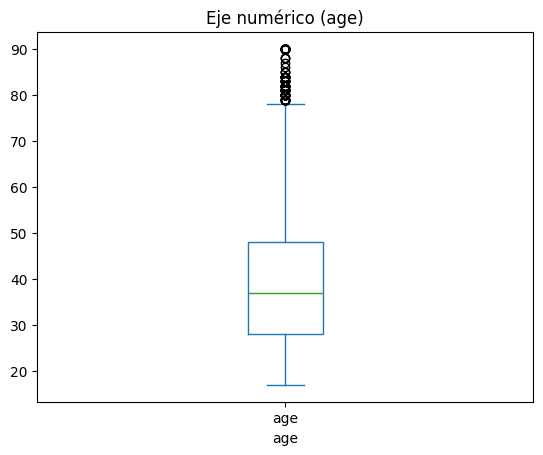
\includegraphics[width=0.8\textwidth]{age.png}  
	\end{figure}
	
	Podemos observar que este eje tiene datos atípicos (outliers) y podríamos estratificar la edad o tomarla como una variable continua o normalizada, por ejemplo, de la menor a la mayor edad o por segmentos de edades.
	\begin{figure}[H]
		\centering
		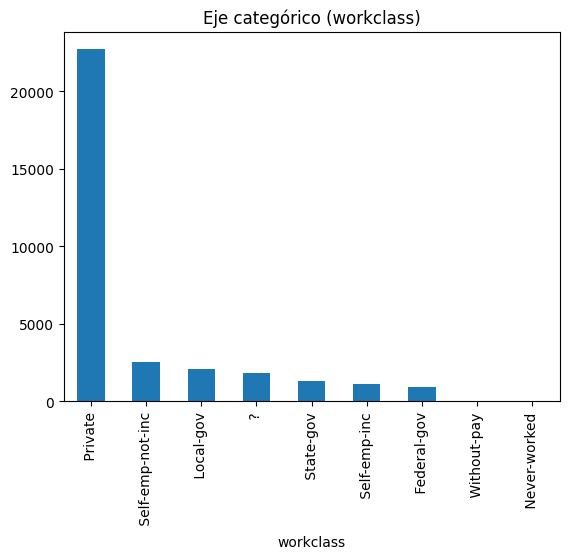
\includegraphics[width=0.8\textwidth]{workclass.png}  
	\end{figure}
	En tipo de trabajo observamos que la mayoría son del sector privado y los demás se dividen en los puestos gubernamentales, auto-empleados y que no trabajan. Además hay una categoría donde están los desconocidos (`?`)
	\begin{figure}[H]
		\centering
		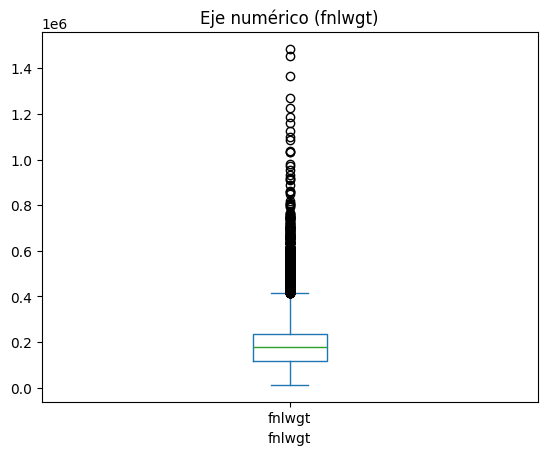
\includegraphics[width=0.8\textwidth]{fnlwgt.png}  
	\end{figure}
	En este eje se observan bastantes datos atípicos.
	\begin{figure}[H]
		\centering
		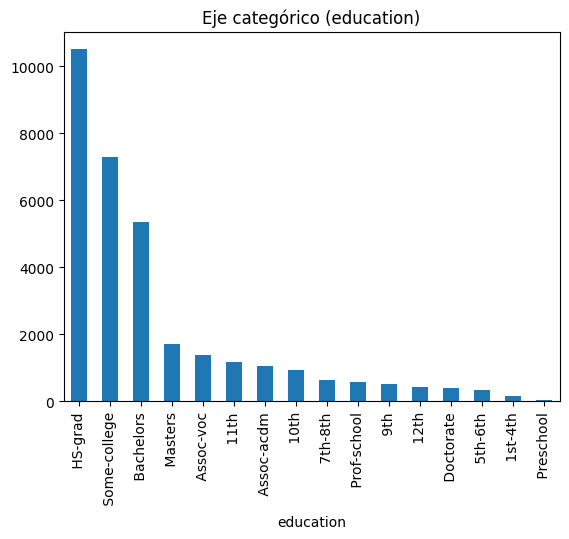
\includegraphics[width=0.8\textwidth]{education.png}  
	\end{figure}
	La categoría con mayor frecuencia son los que tienen educación media superior o preparatoria (HS-grad)
	\begin{figure}[H]
		\centering
		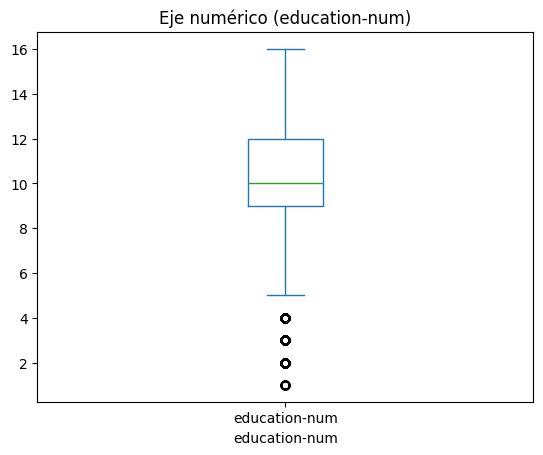
\includegraphics[width=0.8\textwidth]{education-num.png}  
	\end{figure}
	
	\begin{figure}[H]
		\centering
		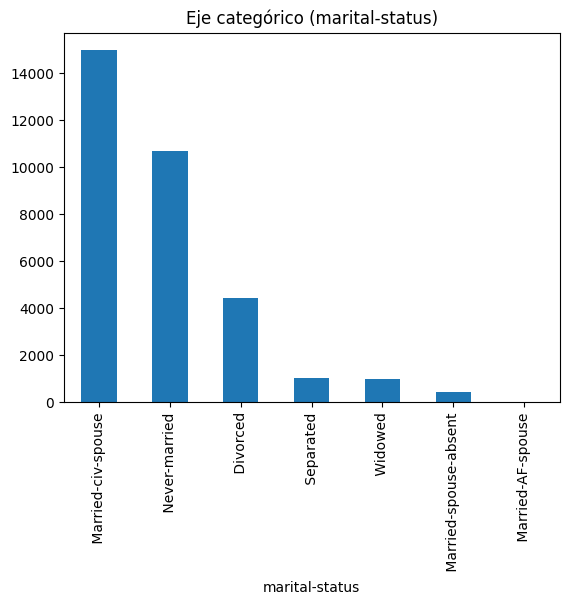
\includegraphics[width=0.8\textwidth]{marital-status.png}  
	\end{figure}
	
	En el estado marital se observa que predominan los que están casados por el civil
	
	\begin{figure}[H]
		\centering
		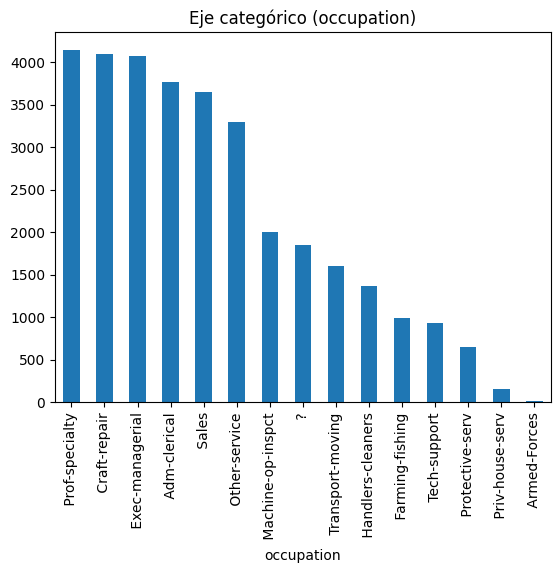
\includegraphics[width=0.8\textwidth]{ocupation.png}  
	\end{figure}
	
	\begin{figure}[H]
		\centering
		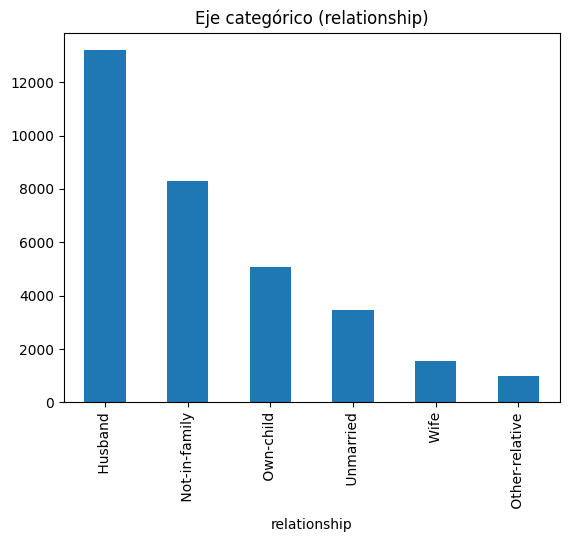
\includegraphics[width=0.8\textwidth]{relationship.png}  
	\end{figure}
	
	Observamos que predomina la categoría esposos.
	
	\begin{figure}[H]
		\centering
		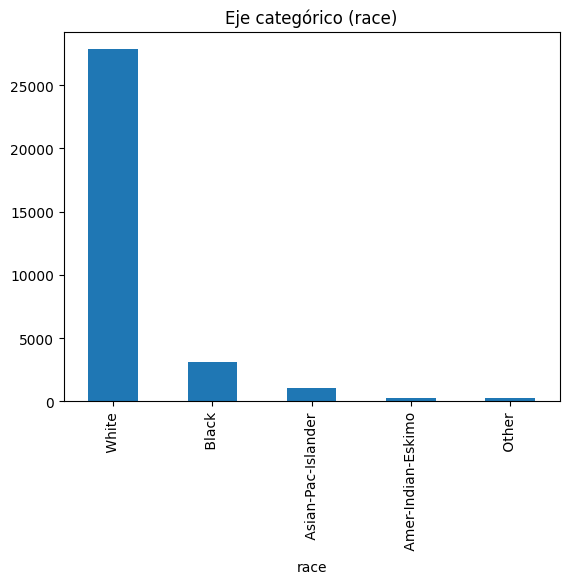
\includegraphics[width=0.8\textwidth]{race.png}
	\end{figure}
	
	La mayoría de las personas son blancas
	
	\begin{figure}[H]
		\centering
		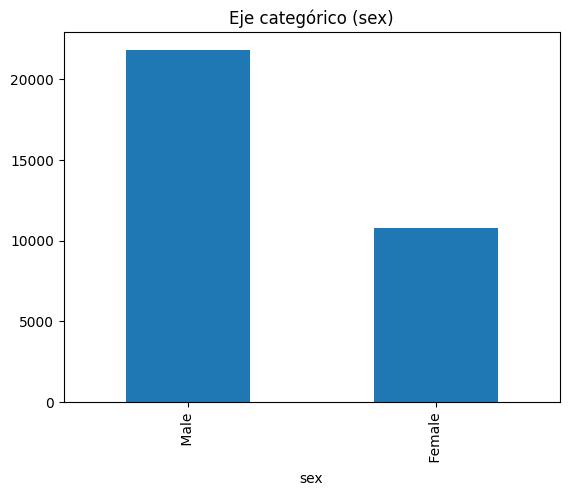
\includegraphics[width=0.8\textwidth]{sex.png}
	\end{figure}
	
	Se observa que son más hombres que mujeres, practicamente el doble.
	
	\begin{figure}[H]
		\centering
		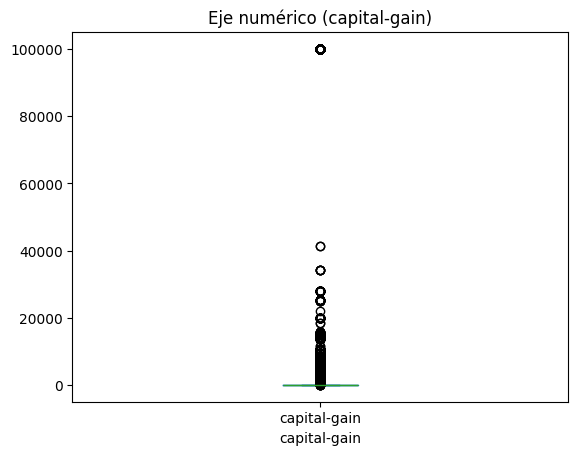
\includegraphics[width=0.8\textwidth]{capital-gain.png}  
	\end{figure}
	
	\begin{figure}[H]
		\centering
		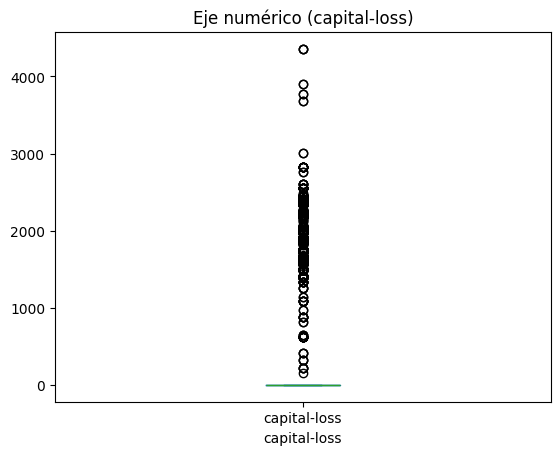
\includegraphics[width=0.8\textwidth]{capital-loss.png}  
	\end{figure}
	Tanto la plusvalía (capital-gain) como la minusvalía (capital-loss) tienen puntos atípicos
	\begin{figure}[H]
		\centering
		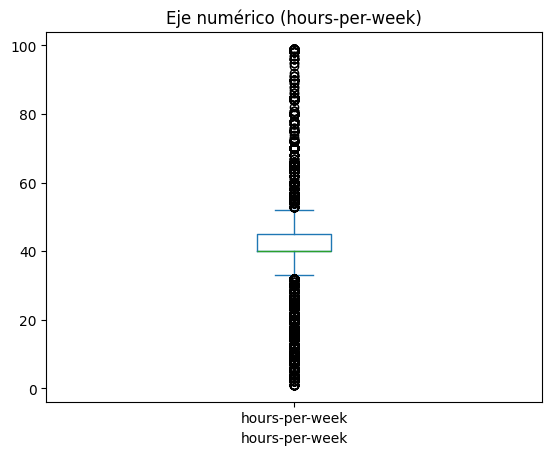
\includegraphics[width=0.8\textwidth]{hours-per-week.png}  
	\end{figure}
	
	
	\begin{figure}[H]
		\centering
		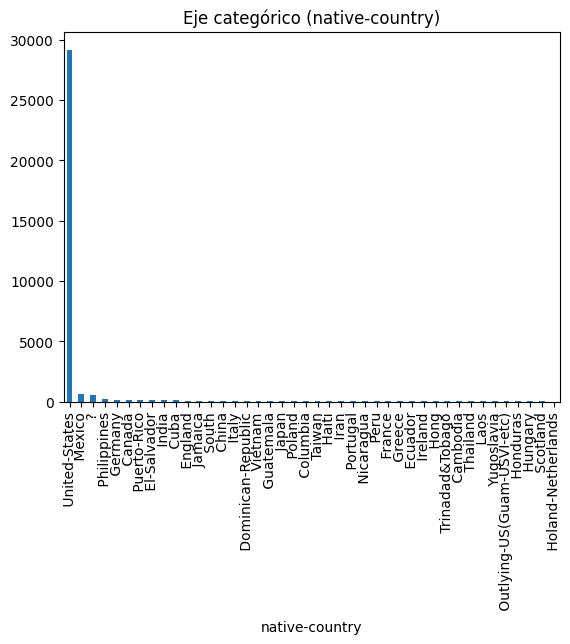
\includegraphics[width=0.8\textwidth]{native-country.png}  
	\end{figure}
	El país con mayor frecuencia son los E.U.A
	\begin{figure}[H]
		\centering
		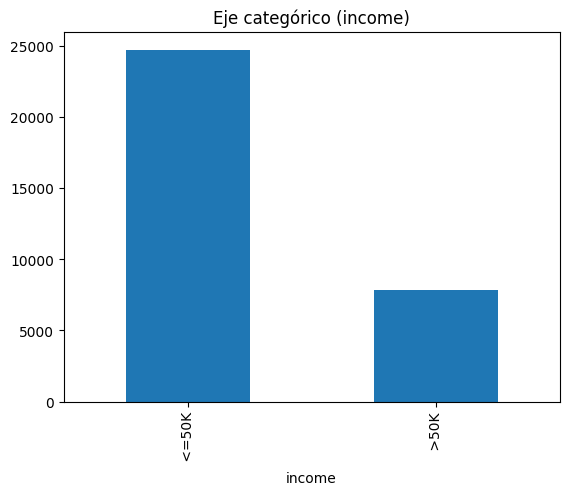
\includegraphics[width=0.8\textwidth]{income.png}  
	\end{figure}
	La mayor parte de las personas gana menos de 50000 dólares al año.
	
	\subsection{Mean encoding (centrado)}
	
	Procedemos a realizar la codificación para las variables categóricas, en este caso usaremos mean encoding centrado ya que esta codificación realiza un contraste direcatemente con la base, es decir la base cero para cada categoría es aquella categoría con mayor frecuencia, a continuación explicamos en que consiste:
	
	\begin{itemize}
		\item Se elige una categoría base (por ejemplo, la más frecuente o la de mayor peso).
		
		\item Se calcula la media global $\mu$ y la media de cada categoría $\mu_j$
	
		\item En vez de usar $\mu_j$ directamente, se usa 
		$\mu_j-\mu_{\text{base}}$
		
		\item Así, la base queda con (efecto cero), y el resto refleja el desvío respecto a ella.
	\end{itemize}
	
	Generamos las gráficas respecto a la diferencia de medias para cada categoría
	
	\begin{figure}[H]
		\centering
		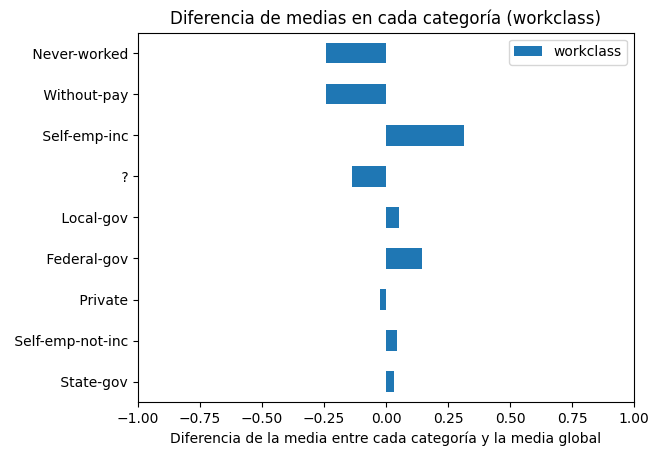
\includegraphics[width=0.8\textwidth]{media_workclass.png}
	\end{figure}
	
	Para esta categoría tomamos como base cero a: Local-gov, Private, Self-emp-not-inc, State-gov ya que la diferencia esta muy cernana a cero
	
	\begin{figure}[H]
		\centering
		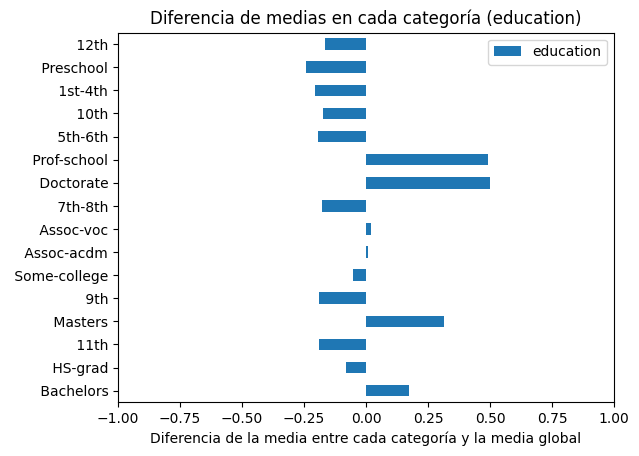
\includegraphics[width=0.8\textwidth]{media_education.png}
	\end{figure}
	En este caso la base cero fue: Assoc-Voc, Assoc-acdm, y en las demás se realizó de forma analoga.
	\begin{figure}[H]
		\centering
		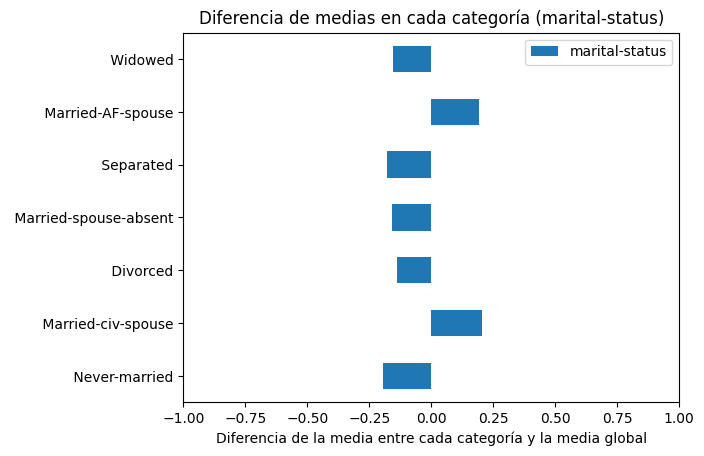
\includegraphics[width=0.8\textwidth]{media_marital.png}
	\end{figure}
	
	\begin{figure}[H]
		\centering
		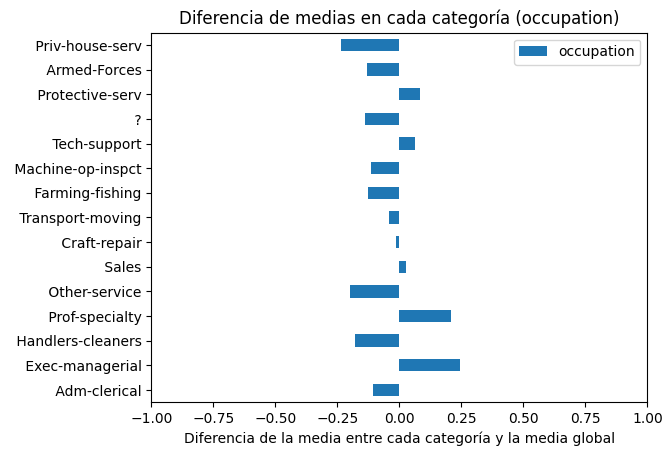
\includegraphics[width=0.8\textwidth]{media_ocupation.png}
	\end{figure}
	
	\begin{figure}[H]
		\centering
		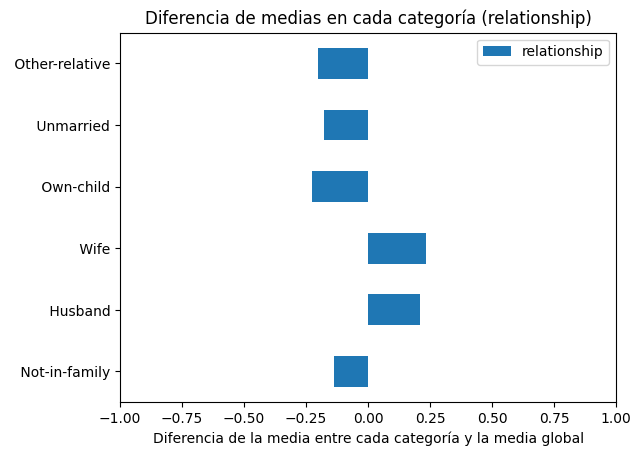
\includegraphics[width=0.8\textwidth]{media_relationship.png}
	\end{figure}
	
	\begin{figure}[H]
		\centering
		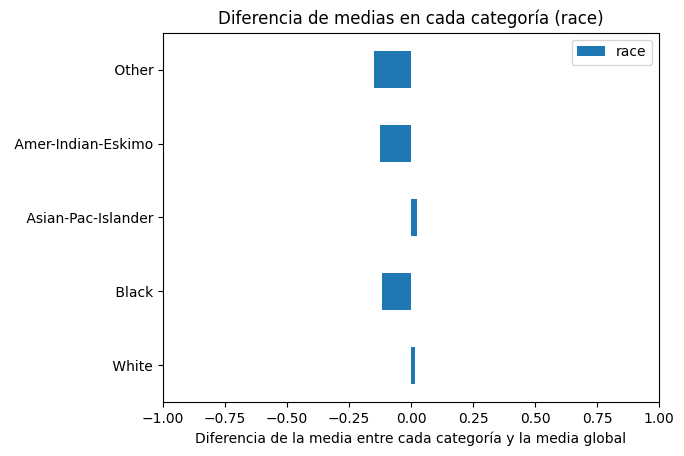
\includegraphics[width=0.8\textwidth]{media_race.png}
	\end{figure}
	
	\begin{figure}[H]
		\centering
		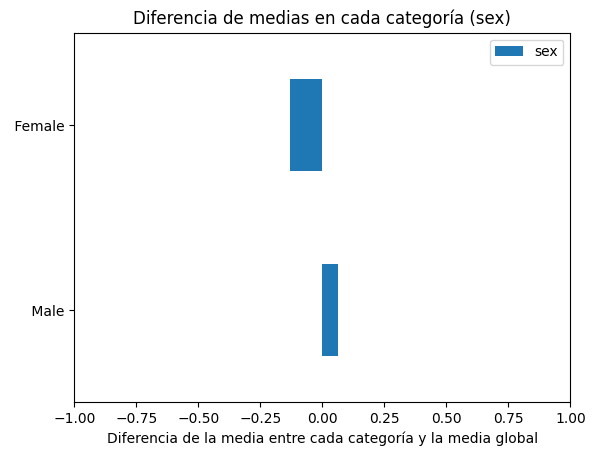
\includegraphics[width=0.8\textwidth]{media_sex.png}
	\end{figure}
	
	
	Una vez terminado la codificación mean encoding centrado, llegamos a un modelo con 27 covariables
	
	
	\section{Análisis - Modelos de Clasificación}
	
	En esta sección utilizamos los modelos de regresión logística, regresión logística Ridge, regresión logística Lasso, Naive Bayes Árboles de decisión, Bosques aleatorios, XGBoost y Support vectorial 
	
	Teniendo en cuenta las siguientes métricas:
	
	Exactitud
	Proporción de predicciones correctas sobre el total de casos.
	
	$$
	\text{Accuracy} = \frac{TP + TN}{TP + TN + FP + FN}
	$$
	
	Precisión (Precision)
	Qué proporción de las predicciones positivas fueron correctas.
	$$
	\text{Precision} = \frac{TP}{TP + FP}
	$$
	
	Sensibilidad (Recall o TPR)
	Qué proporción de los positivos reales fueron correctamente identificados.
	$$
	\text{Recall} = \frac{TP}{TP + FN}
	$$
	
	Especificidad (TNR)
	Qué proporción de los negativos reales fueron correctamente identificados.
	$$
	\text{Specificity} = \frac{TN}{TN + FP}
	$$
	
	F1-score
	Media armónica entre precisión y recall.
	$$
	\text{F1} = 2 \times \frac{\text{Precision} \times \text{Recall}}{\text{Precision} + \text{Recall}}
	$$
	
	La matriz de confusión esta dada por:
	\[\text{Matriz de Confusión}=
	\begin{bmatrix}
		TN & FP \\
		FN & TP
	\end{bmatrix}
	\]
	
	donde:
	\begin{itemize}
		\item TN: True Negatives (verdaderos negativos)
		\item FP: False Positives (falsos positivos)
		\item FN: False Negatives (falsos negativos)
		\item TP: True Positives (verdaderos positivos)
	\end{itemize}
	
	Resultados
	odemos observar la diferencia de la exactitud y el área bajo la curva ROC de los diferentes modelos:
	
	\begin{table}[ht]
		\centering
		\begin{tabular}{|l|c|c|}
			\hline
			\textbf{Modelo} & \textbf{Exactitud} & \textbf{AUC} \\
			\hline
			Logístico Simple  & 0.76 & 0.51 \\
			Logístico Lasso   & 0.76 & 0.51 \\
			Logístico Ridge   & 0.76 & 0.51 \\
			Naive Bayes       & 0.83 & 0.87 \\
			Árbol de Decisión & 0.79 & 0.72 \\
			Bosque Aleatorio  & 0.83 & 0.88 \\
			XGBoost           & 0.85 & 0.90 \\
			Support Vector    & 0.85 & 0.90 \\
			\hline
		\end{tabular}
		\caption{Comparación de modelos de clasificación}
		\label{tab:modelos}
	\end{table}
	
	Dado que los mejores modelos son XGBoost y Support vectorial, decidimos quedarnos con el modelo XGBoost para entrenarlo y realizar la clasificación.
	
	\section{Entrenamiento, validación cruzada del modelo XGBoost y Resultados}
	
	Utilizamos la técnica de búsqueda aleatoria para encontrar los hiperparámetros óptimos para realizar la clasificación, finalmente la exactitud (accuracy) obtenido para el modelo de clasificación usando XGBoost fue de $0.853$
	
	\begin{figure}[H]
		\centering
		\includegraphics[width=0.8\textwidth]{matriz_XGBoost.png}
	\end{figure}
	
	
	\begin{table}[ht]
		\centering
		\begin{tabular}{|l|c|}
			\hline
			\textbf{Métrica} & \textbf{Valor} \\
			\hline
			Exactitud     & 0.852910 \\
			Precisión     & 0.740536 \\
			Sensibilidad  & 0.598852 \\
			Especificidad & 0.933468 \\
			F1-Score      & 0.662200 \\
			\hline
		\end{tabular}
		\caption{Métricas de desempeño del modelo XGBoost optimizado}
		\label{tab:metricas_xgboost}
	\end{table}
	
	
	\section{Conclusiones}
	
	Al final el modelo de clasificación nos dió un alto rendimiento predictivo, el modelo XGBoost logró una exactitud del 85.3\%, lo que indica un desempeño sólido al predecir si una persona gana más o menos de \$50,000 al año, esto indica que las características socioeconómicas contenidas en el dataset tienen buen poder predictivo respecto al ingreso. De la matriz de confusión concluimos lo siguiente:
	
	\begin{itemize}
		\item Una precisión de 74.1\% implica que, entre las personas que el modelo predice como de altos ingresos, el 74.1\% realmente pertenece a esa categoría.
		
		\item La sensibilidad (59.9\%) muestra que el modelo detecta correctamente a casi el 60\% de las personas que efectivamente ganan más de \$50,000, lo cual es aceptable pero deja espacio para mejoras si el objetivo es minimizar falsos negativos.
		
		\item La especificidad elevada (93.3\%) indica que el modelo distingue con gran eficacia a las personas que no ganan más de \$50,000.
		
		\item El F1-score de 66.2\% representa un equilibrio razonable entre precisión y sensibilidad, especialmente útil si existe cierto desbalance entre clases.
		
	\end{itemize}
	
	
	En conjunto, estos resultados reflejan un modelo que generaliza bien, con una alta capacidad para evitar falsos positivos, y un desempeño sólido que puede servir como base confiable en aplicaciones prácticas.
	
	\newpage
	
	\section{Anexo: C\'odigo en Python para Clasificaci\'on del Dataset Adult}
	
	\begin{lstlisting}[language=Python]
		import numpy
		import pandas
		import matplotlib.pyplot as pyplot
		import seaborn
		
		adult = pandas.read_csv("adult.data", header=None)
		
		adult.columns = [
		"age", "workclass", "fnlwgt", "education", "education-num", "marital-status",
		"occupation", "relationship", "race", "sex", "capital-gain", "capital-loss",
		"hours-per-week", "native-country", "income"]
		
		adult.info()
		
		for column in adult.columns:
		if adult[column].dtype == object:
		adult[column].value_counts().plot.bar()
		pyplot.xlabel(column)
		pyplot.title(f"Eje categ\'orico ({column})")
		pyplot.show()
		else:
		adult[column].plot.box()
		pyplot.xlabel(column)
		pyplot.title(f"Eje num\'erico ({column})")
		pyplot.show()
		
		y = adult["income"].map({" <=50K": 0, " >50K": 1})
		
		for column in adult.columns:
		if column == "native-country" or column == "income":
		continue
		if adult[column].dtype != object:
		continue
		
		mu = y.mean()
		categorias = adult[column].unique()
		xj = pandas.DataFrame(numpy.zeros(len(categorias)), index=categorias, columns=[column])
		
		for cat_j in categorias:
		mu_j = y[adult[column] == cat_j].mean()
		xj.loc[cat_j] = mu_j - mu
		
		xj.plot.barh()
		pyplot.title(f"Diferencia de medias en cada categor\'ia ({column})")
		pyplot.xlabel("Diferencia de la media entre cada categor\'ia y la media global")
		pyplot.xlim((-1, 1))
		pyplot.show()
		
		mu = y.mean()
		categorias = adult["native-country"].unique()
		xj = pandas.DataFrame(numpy.zeros_like(categorias), index=categorias, columns=["native-country"])
		
		for cat_j in categorias:
		mu_j = y[adult["native-country"] == cat_j].mean()
		xj.loc[cat_j] = mu_j - mu
		
		xj.plot.bar()
		
		from sklearn.cluster import KMeans
		clu = KMeans()
		clu.fit(xj)
		xj["clu"] = clu.labels_
		
		def test_categorias(x, indices=[]):
		categorias = x.unique()
		s = numpy.zeros_like(x)
		for j in indices:
		cat_j = categorias[j]
		s = s + (x == cat_j).astype(int)
		return s
		
		x1 = test_categorias(adult["workclass"], [8, 7])
		x2 = test_categorias(adult["workclass"], [6])
		x3 = test_categorias(adult["workclass"], [3])
		x4 = test_categorias(adult["workclass"], [4, 0, 1])
		x5 = test_categorias(adult["workclass"], [5])
		
		x6 = test_categorias(adult["education"], [9, 10])
		x7 = test_categorias(adult["education"], [3, 0])
		x8 = test_categorias(adult["education"], [14, 13, 11])
		x9 = test_categorias(adult["education"], [8, 4, 12, 2, 15])
		
		x10 = test_categorias(adult["marital-status"], [5, 1])
		
		x11 = test_categorias(adult["occupation"], [14, 4, 2])
		x12 = test_categorias(adult["occupation"], [3, 1])
		x13 = test_categorias(adult["occupation"], [12, 10, 5])
		x14 = test_categorias(adult["occupation"], [2, 1])
		x15 = test_categorias(adult["race"], [4, 3, 1])
		x16 = test_categorias(adult["sex"], [1])
		x17 = test_categorias(adult["native-country"], [12, 26, 3, 21, 29, 30, 17])
		x18 = test_categorias(adult["native-country"], [14, 9, 10, 11, 13, 38])
		x19 = test_categorias(adult["native-country"], [18, 19, 2, 20, 23, 34, 7, 22])
		x20 = test_categorias(adult["native-country"], [25, 8, 37, 31, 36, 5, 27])
		x21 = test_categorias(adult["native-country"], [16, 24, 32, 41])
		
		def winzorizado(x):
		Q1 = x.quantile(0.25)
		Q3 = x.quantile(0.75)
		IQR = Q3 - Q1
		xmin = Q1 - 1.5 * IQR
		xmax = Q3 + 1.5 * IQR
		xp = (x < xmin) * xmin + ((x >= xmin) & (x <= xmax)) * x + (x > xmax) * xmax
		return xp
		
		x22 = winzorizado(adult["age"])
		x23 = winzorizado(adult["fnlwgt"])
		x24 = winzorizado(adult["education-num"])
		x25 = (adult["capital-gain"] > 0).astype(int)
		x26 = (adult["capital-loss"] > 0).astype(int)
		x27 = winzorizado(adult["hours-per-week"])
		
		X = pandas.DataFrame([
		x1, x2, x3, x4, x5, x6, x7, x8, x9, x10,
		x11, x12, x13, x14, x15, x16, x17, x18, x19, x20,
		x21, x22, x23, x24, x25, x26, x27
		], index=[
		"x1", "x2", "x3", "x4", "x5", "x6", "x7", "x8", "x9", "x10",
		"x11", "x12", "x13", "x14", "x15", "x16", "x17", "x18", "x19", "x20",
		"x21", "x22", "x23", "x24", "x25", "x26", "x27"
		]).T
		
		from sklearn.model_selection import train_test_split
		from sklearn.metrics import confusion_matrix, roc_curve, auc
		from sklearn.linear_model import LogisticRegression
		from sklearn.naive_bayes import BernoulliNB
		from sklearn.tree import DecisionTreeClassifier
		from sklearn.ensemble import RandomForestClassifier
		from sklearn.svm import SVC
		from xgboost import XGBClassifier
		from sklearn.model_selection import RandomizedSearchCV
		from sklearn.metrics import accuracy_score
		import seaborn as sns
		import matplotlib.pyplot as plt
		
		X_train, X_test, y_train, y_test = train_test_split(X, y,
		train_size=0.8, random_state=123, stratify=y)
		
		cv = RandomizedSearchCV(
		XGBClassifier(),
		param_distributions={
			"max_depth": [None, 10, 100],
			"max_leaves": [4, 6, 8]
		}
		)
		
		cv.fit(X_train, y_train)
		mejores_params = cv.best_params_
		
		clf_optimizado = XGBClassifier(
		**mejores_params,
		eval_metric="logloss",
		random_state=123
		)
		
		clf_optimizado.fit(X_train, y_train)
		y_pred = clf_optimizado.predict(X_test)
		
		C = confusion_matrix(y_test, y_pred)
		TN, FP, FN, TP = C.ravel()
		
		plt.figure(figsize=(6, 4))
		sns.heatmap(C, annot=True, fmt="d", cmap="coolwarm", xticklabels=["<=50K", ">50K"], yticklabels=["<=50K", ">50K"])
		plt.xlabel("Predicci\'on")
		plt.ylabel("Valor Real")
		plt.title("Matriz de Confusi\'on - XGBoost Optimizado")
		plt.show()
		
		exactitud = (TN + TP) / (TN + FP + FN + TP)
		precision = TP / (TP + FP)
		sensibilidad = TP / (TP + FN)
		especificidad = TN / (TN + FP)
		f1 = 2 * (precision * sensibilidad) / (precision + sensibilidad)
		
		pd.DataFrame(
		[exactitud, precision, sensibilidad, especificidad, f1],
		index=["Exactitud", "Precisi\'on", "Sensibilidad", "Especificidad", "F1-Score"],
		columns=["Valor"]
		)
	\end{lstlisting}
	
	
	
\end{document}
